\documentclass[12pt, letterpaper]{article}
\usepackage{amsthm, amsmath, amssymb, graphicx, hyperref, url, pdfpages}
\usepackage[utf8]{inputenc}
\usepackage{pgfplots}
\pgfplotsset{compat=1.18}

\newtheorem{thm}{Theorem}[section]
\newtheorem{lemma}[thm]{Lemma}

\theoremstyle{definition}
\newtheorem{ex}[thm]{Example}
\newtheorem{defn}[thm]{Definition}

\title{The Quadratic Formula}
\author{Gordon Chen}
\date{Fall 2026}

\begin{document}
\maketitle

\section{Introduction} \label{intro}
In this paper we will show how to derive the quadratic formula \cite{wiki:quadratic_formula}
and use it to find the roots \cite{wiki:roots} of
quadratic functions \cite{wiki:quadratic_equation}.

In Section \ref{sec2} we will define some preliminaries related to quadratic functions
and their roots.

In Section \ref{sec3} we will provide a proof that the roots of quadratic functions are
given by the quadratic formula.

Finally, in Section \ref{sec4} we will see some examples of the quadratic formula in action.


\section{Preliminaries} \label{sec2}
\begin{defn}
  A quadratic (function) is a polynomial \cite{wiki:polynomial}
  of degree 2. A quadratic has the following form:
    \[ f(x) = a x^2 + bx + c, \]
    where \(a, b, c \in \mathbb{R}\) and \(a \ne 0\).
\end{defn}

\begin{defn}
    Let \(x \in \mathbb{R}\). Then \(x\) is a real root of the quadratic \(f\) if \(f(x) = 0\).
\end{defn}

\begin{defn}
  The quadratic formula is \[ x = \frac{-b \pm \sqrt{b^2 - 4 a c}}{2a} \]
  when \(a, b, c \in \mathbb{R}\), \(a \ne 0\), and \(b^2 - 4 a c \ge 0\) so that the square root
  is defined.
\end{defn}

\section{Proof} \label{sec3}
\begin{thm}
    Let \(a, b, c \in \mathbb{R}\) and \(a \ne 0\).
    Let \(f\) be the quadratic given by \(f(x) = a x^2 + bx + c\).
    Then \(x \in \mathbb{R}\) is a root of \(f\) if and only if \(x\) satisfies the
    quadratic formula.

    \begin{proof}
        Let \(a, b, c \in \mathbb{R}\) and \(a \ne 0\).
        Let \(f\) be the quadratic given by \(f(x) = a x^2 + bx + c.\) \\

        First we check that if \(x=\frac{-b \pm \sqrt{b^2 - 4 a c}}{2a}\), and \(b^2 - 4ac \ge 0\)
        so that the square root is defined and \(x \in \mathbb{R}\),
        then \(x\) is a root of \(f\).

        Let \(x = \frac{-b + \sqrt{b^2 - 4 a c}}{2a}\).
        Then we have the following:
        \begin{align*}
        f(x) &= a \left(\frac{-b + \sqrt{b^2 - 4 a c}}{2a}\right)^2
                + b \left(\frac{-b + \sqrt{b^2 - 4 a c}}{2a}\right) + c \\
             &= a \frac{\left(-b + \sqrt{b^2 - 4 a c}\right)^2}{\left(2a\right)^2}
                + \frac{-b^2 + b\sqrt{b^2 - 4 a c}}{2a} + c \\
             &= a \frac{b^2 - 2b \sqrt{b^2 - 4 a c} + b^2 - 4 a c}{4a^2}
                + \frac{-b^2 + b\sqrt{b^2 - 4 a c}}{2a} + c \\
             &= \frac{2 a b^2 - 2ab \sqrt{b^2 - 4 a c} - 4 a^2 c}{4a^2}
                + \frac{-b^2 + b\sqrt{b^2 - 4 a c}}{2a} + c \\
             &= \frac{2 a b^2 - 2ab \sqrt{b^2 - 4 a c} - 4 a^2 c}{4a^2}
             + \frac{-2ab^2 + 2ab\sqrt{b^2 - 4 a c}}{4a^2} + \frac{4a^2c}{4a^2} \\
             &= \frac{2 a b^2 - 2ab \sqrt{b^2 - 4 a c} - 4 a^2 c
                -2ab^2 + 2ab\sqrt{b^2 - 4 a c} + 4a^2c}{4a^2} \\
             &= \frac{2 a b^2 -2ab^2 + 2ab\sqrt{b^2 - 4 a c} - 2ab \sqrt{b^2 - 4 a c}
                + 4a^2c  - 4 a^2 c}{4a^2} \\
             &= \frac{0}{4a^2} \\
             &= 0.
        \end{align*}

        Now we consider the other root given by the quadratic formula, when
        \(x = \frac{-b - \sqrt{b^2 - 4 a c}}{2a}\).
        Then we have the following:

        \begin{align*}
        f(x) &= a \left(\frac{-b - \sqrt{b^2 - 4 a c}}{2a}\right)^2
                + b \left(\frac{-b - \sqrt{b^2 - 4 a c}}{2a}\right) + c \\
             &= a \frac{\left(-b - \sqrt{b^2 - 4 a c}\right)^2}{\left(2a\right)^2}
                + \frac{-b^2 - b\sqrt{b^2 - 4 a c}}{2a} + c \\
             &= a \frac{b^2 + 2b \sqrt{b^2 - 4 a c} + b^2 - 4 a c}{4a^2}
                + \frac{-b^2 - b\sqrt{b^2 - 4 a c}}{2a} + c \\
             &= \frac{2 a b^2 + 2ab \sqrt{b^2 - 4 a c} - 4 a^2 c}{4a^2}
                + \frac{-b^2 - b\sqrt{b^2 - 4 a c}}{2a} + c \\
             &= \frac{2 a b^2 + 2ab \sqrt{b^2 - 4 a c} - 4 a^2 c}{4a^2}
             + \frac{-2ab^2 - 2ab\sqrt{b^2 - 4 a c}}{4a^2} + \frac{4a^2c}{4a^2} \\
             &= \frac{2 a b^2 + 2ab \sqrt{b^2 - 4 a c} - 4 a^2 c
                -2ab^2 - 2ab\sqrt{b^2 - 4 a c} + 4a^2c}{4a^2} \\
             &= \frac{2 a b^2 -2ab^2 + 2ab\sqrt{b^2 - 4 a c} - 2ab \sqrt{b^2 - 4 a c}
                + 4a^2c  - 4 a^2 c}{4a^2} \\
             &= \frac{0}{4a^2} \\
             &= 0.
        \end{align*}

        So if \(x = \frac{-b \pm \sqrt{b^2 - 4 a c}}{2a}\)
        then \(f(x) = 0\), so \(x\) is a root of \(f\). \\

        Now we check the other direction, that if \(x\) is a root of a polynomial,
        then \[x = \frac{-b \pm \sqrt{b^2 - 4 a c}}{2a}.\]

        We want to solve the equation \(f(x) = 0\). By completing the square
        \cite{wiki:completing_the_square} and solving for \(x\), we get the following:
        \begin{align*}
          0 &= f(x) \\
            &= ax^2 + bx + c \\
            &= x^2 + \frac{b}{a}x + \frac{c}{a} \\
            &= x^2 + \frac{b}{a}x + \left(\frac{b}{2a}\right)^2 - \left(\frac{b}{2a}\right)^2
            + \frac{c}{a} \\
          0 &= \left(x + \frac{b}{2a}\right)^2 + \frac{c}{a} - \frac{b^2}{4a^2} \\
          \left(x + \frac{b}{2a}\right)^2 =& \frac{b^2}{4a^2} - \frac{c}{a} \\
          \left(x + \frac{b}{2a}\right)^2 =& \frac{b^2 - 4a c}{4a^2}\\
          x + \frac{b}{2a} =& \pm \sqrt{\frac{b^2 - 4a c}{4a^2}} \\
          x + \frac{b}{2a} =& \frac{\pm \sqrt{b^2 - 4a c}}{2|a|} \\
          x =& \frac{-b \pm \sqrt{b^2 - 4a c}}{2a}.
        \end{align*}

        So, we now see that the real roots (if they exist) of the quadratic $f$ are given by the
        quadratic formula \[x = \frac{-b \pm \sqrt{b^2 - 4a c}}{2a}.\]

        If \(b^2 - 4a c > 0\), then we have 2 real roots
        \[x = \frac{-b \pm \sqrt{b^2 - 4a c}}{2a}.\]

        If \(b^2 - 4a c = 0\), then
        \[x = \frac{-b \pm \sqrt{b^2 - 4a c}}{2a} = \frac{-b \pm \sqrt{0}}{2a} = \frac{-b}{2a}\]
        so the quadratic formula gives us a single real root.

        Finally, if \(b^2 - 4a c < 0\), then \(\sqrt{b^2 - 4ac}\) is not real, so
        the quadratic has no real roots. \\

        So we first showed that if \(x\) satisfies the quadratic formula, then \(x\) is a root
        of the quadratic.
        Then we showed that if \(x\) is a root of a quadratic, then \(x\) satisfies the quadratic
        formula. Thus, \(x\) is a root of a quadratic if and only if \(x\) satisfies the
        quadratic formula.
    \end{proof}
\end{thm}


\section{Examples} \label{sec4}

\begin{ex}
  Let \(f(x) = 2x^2 + 6x + 4\).

  By the quadratic formula, the roots of \(f\) are
  \begin{align*}
  x &= \frac{-b \pm \sqrt{b^2 - 4ac}}{2a} \\
    &= \frac{-6 \pm \sqrt{6^2 - 4(2)(4)}}{2(2)} \\
    &= \frac{-6 \pm \sqrt{36 - 32}}{4} \\
    &= \frac{-6 \pm \sqrt{4}}{4} \\
    &= \frac{-6 \pm 2}{4} \\
    &= \frac{-4}{4} \text{ or } \frac{-8}{4} \\
    &= -1 \text{ or } -2.
  \end{align*}

  Now we check:
  \begin{align*}
    f(-1) &= 2(-1)^2 + 6(-1) + 4 = 2 - 6 + 4 = 0 \\
    f(-2) &= 2(-2)^2 + 6(-2) + 4 = 2(4) - 12 + 4 = 8 - 12 + 4 = 0.
  \end{align*}

  So we have verified that \(x=-1\) and \(x=-2\) given by the quadratic formula
  are indeed roots of \(f\).

  This is an example of a quadratic with 2 real roots. This is consistent with the condition
  we saw in Section \ref{sec3}, that a quadratic has 2 real roots if \(b^2 - 4a c > 0\),
  which this quadratic satisfies since \(6^2 - 4(2)(4) = 36 - 32 = 4 > 0\).

  \begin{figure}[ht]
      \centering
      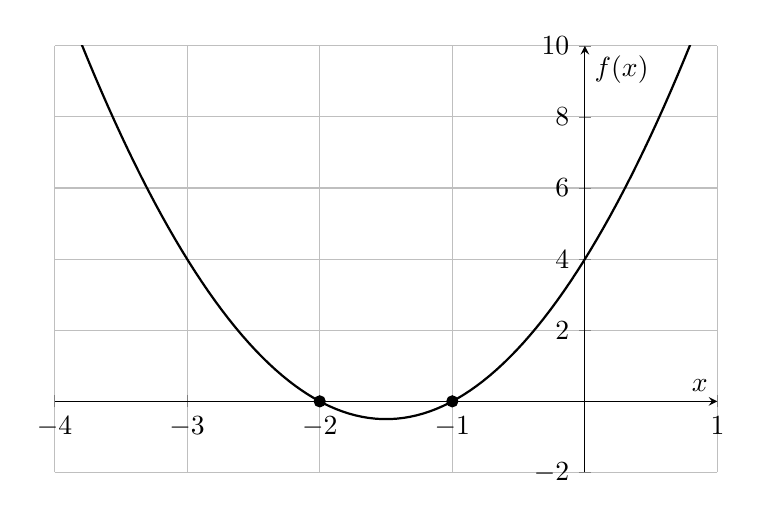
\begin{tikzpicture}
          \begin{axis}[
              axis lines=middle,
              xlabel={$x$},
              ylabel={$f(x)$},
              xmin=-4, xmax=1,
              ymin=-2, ymax=10,
              samples=100,
              grid=both,
              width=10cm,
              height=7cm,
          ]
              \addplot[thick, domain=-4:1] {2*x^2 + 6*x + 4};
              \addplot[only marks, mark=*] coordinates {(-2,0) (-1,0)};
              \node[below] at (axis cs:-2,0) {};
              \node[below] at (axis cs:-1,0) {};
          \end{axis}
      \end{tikzpicture}
      \caption{The graph of $f(x)=2x^2+6x+4$.}
      \label{fig:graph1}
  \end{figure}

  Plotting the quadratic in Figure \ref{fig:graph1} we can also see that it indeed has 2 roots, one at \(x=-2\) and
  the other at \(x=-1\).
\end{ex}


\begin{ex}
  Let \(f(x) = x^2 + 2x + 1\).

  By the quadratic formula, the roots of \(f\) are
  \begin{align*}
  x &= \frac{-b \pm \sqrt{b^2 - 4ac}}{2a} \\
    &= \frac{-2 \pm \sqrt{2^2 - 4(1)(1)}}{2(1)} \\
    &= \frac{-2 \pm \sqrt{4 - 4}}{2} \\
    &= \frac{-2}{2} \\
    &= -1.
  \end{align*}

  Now we check:
  \begin{align*}
    f(-1) &= (-1)^2 + 2(-1) + 1 = 1 - 2 + 1 = 0
  \end{align*}

  So we have verified that \(x=-1\) given by the quadratic formula is indeed a root of \(f\).

  This is an example of a quadratic with a single real roots.
  This is consistent with the condition we saw in Section \ref{sec3},
  that a quadratic has only one real roots if \(b^2 - 4a c = 0\),
  which this quadratic satisfies since \(2^2 - 4(1)(1) = 4 - 4 = 0\).

  \begin{figure}[ht]
      \centering
      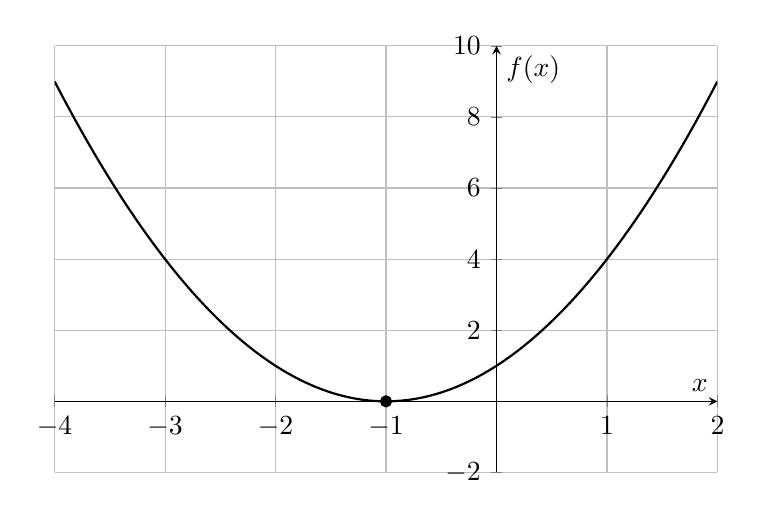
\begin{tikzpicture}
          \begin{axis}[
              axis lines=middle,
              xlabel={$x$},
              ylabel={$f(x)$},
              xmin=-4, xmax=2,
              ymin=-2, ymax=10,
              samples=100,
              grid=both,
              width=10cm,
              height=7cm,
          ]
              \addplot[thick, domain=-4:2] {x^2 + 2*x + 1};
              \addplot[only marks, mark=*] coordinates {(-1,0)};
              \node[below] at (axis cs:-1,0) {};
          \end{axis}
      \end{tikzpicture}
      \caption{The graph of $f(x)=x^2+2x+1$.}
      \label{fig:graph2}
  \end{figure}

  Plotting the quadratic in Figure \ref{fig:graph2} we can also see that it indeed has only
  one real root \(x=-1\).
\end{ex}


\begin{ex}
  Let \(f(x) = x^2 + 2x + 2\).

  By the quadratic formula, the roots of \(f\) are
  \begin{align*}
  x &= \frac{-b \pm \sqrt{b^2 - 4ac}}{2a} \\
    &= \frac{-2 \pm \sqrt{2^2 - 4(1)(2)}}{2(1)} \\
    &= \frac{-2 \pm \sqrt{4 - 8}}{2} \\
    &= \frac{-2 \pm \sqrt{-4}}{2} \\
  \end{align*}

  But \(\sqrt{-4}\) is imaginary so this quadratic has no real roots.
  This is consistent with the condition we saw in Section \ref{sec3},
  that a quadratic has no real roots if \(b^2 - 4a c < 0\),
  which this quadratic satisfies since \(2^2 - 4(1)(2) = 4 - 8 = -4 < 0\).

  \begin{figure}[ht]
      \centering
      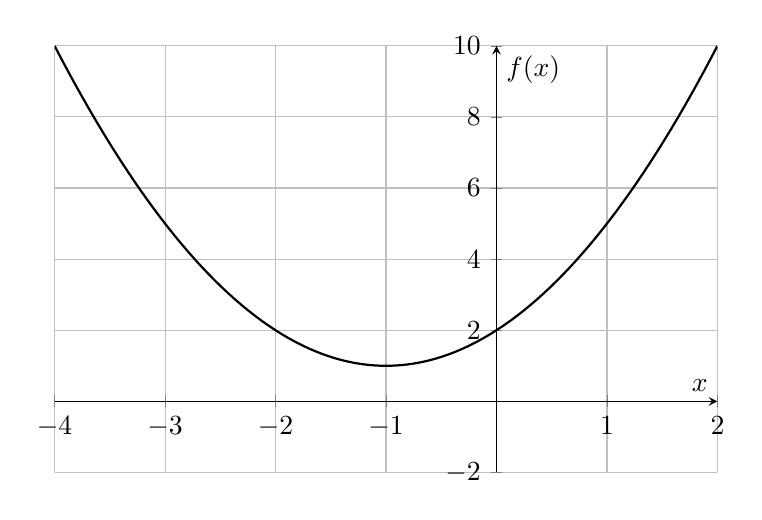
\begin{tikzpicture}
          \begin{axis}[
              axis lines=middle,
              xlabel={$x$},
              ylabel={$f(x)$},
              xmin=-4, xmax=2,
              ymin=-2, ymax=10,
              samples=100,
              grid=both,
              width=10cm,
              height=7cm,
          ]
              \addplot[thick, domain=-4:2] {x^2 + 2*x + 2};
          \end{axis}
      \end{tikzpicture}
      \caption{The graph of $f(x)=x^2+2x+2$.}
      \label{fig:graph3}
  \end{figure}

  Plotting the quadratic in Figure \ref{fig:graph3} we can also see that it indeed has
  no real roots (does not touch the x-axis).
\end{ex}


\bibliographystyle{plain}
\bibliography{refs}

% \includepdf[pages=-]{quadratic_feedback.pdf}

\end{document}
